\documentclass{article}

\usepackage{../swiftnav}
\usepackage{../swiftnav_tikz}

\usepackage{endnotes}

\usepackage{draftwatermark}
\SetWatermarkLightness{0.9}
\SetWatermarkText{Preliminary}
\SetWatermarkScale{4}

\newenvironment{mpar}{\par\noindent\minipage{\linewidth}}{\endminipage\par}
%\setlength{\skip\mpfootins}{2cm}
\renewcommand{\thempfootnote}{\arabic{mpfootnote}}

% ---------------------------------------------------------------------------

\version{1.0}
\title{SwiftGNSS Datasheet}
\author{Swift Navigation}
\date{\today}

\begin{document}

\maketitle

\begin{multicols*}{2}
\raggedcolumns

\section*{Features}
\large
\label{sec:Features}
\begin{itemize}
  \bulletnoindent
  \item Open-Source GNSS Receiver Platform.
  \item Flexible architecture.
  \item Carrier-phase RTK capable for centimetre level positioning.
  \item 50Hz navigation solution update rate.
  \item Small form factor.
  \item Very low power consumption.
  \item USB and 2x UART connectivity.
  \item Integrated patch antenna.
  \item Stand-alone operation.
  \item Full-rate sample passthrough over USB.
  \item Single-frequency L1 3-bit, 16.368 MS/s\\RF front-end.
\end{itemize}
\normalsize

\section*{Applications}
\large
\label{sec:Applications}
\begin{itemize}
  \bulletnoindent
  \item GPS/GNSS Research.
  \item Unmanned Aerial Vehicle Guidance.
  \item Autonomous Landing Systems.
  \item Surveying Systems.
\end{itemize}
\normalsize

\section*{Description}

SwiftGPS (working name) is a low-cost, open-source GNSS receiver
platform with RTK capabilities.  It has been built to be flexible,
allowing customization and experimentation at all levels (e.g. raw IF
data, tracking loop filters, PVT solution methods).  It is targeted both for
the GNSS research community and for integration into demanding real-world
applications such as aerobatic UAVs.

The architecture is based around a MAX2769 3-bit 16MS/s front end
attached to a Spartan-6 FPGA which contains correlators specialized
for satellite signal tracking and acquisition, as well as programmable
digital notch filters for CW noise nulling.  The FPGA is connected by
a high speed register-level interface to a Cortex-M4 microprocessor
which performs all functions above the correlator level, including
tracking loop filters, acquisition management and navigation
processing.

The high speed Cortex-M4 processor is capable of processing tracking
channel updates at 1 kHz and producing PVT solutions at better than 50
Hz depending on the navigation filter chosen.

The receiver can operate standalone or be connected via a rich debug
protocol to a PC running a Python graphical console for status
monitoring and rapid prototyping of new algorithms.

At the moment our prototypes are L1-only, but we intend to add dual
frequency capability in the near future.  The correlators are
presently based around a 1023-bit PRN intended for GPS and WAAS C/A
code but could be readily adapted to use with other signals such as
L2C or Galileo.

In the past we have successfully prototyped multi-antenna receiver systems and
used them in RTK mode for control in highly dynamic environments (tethered
UAVs under 12 g acceleration in circular paths, feet above the ground).
Further down the pipeline, we plan to build an advanced platform with
inertial aiding as well as multiple antennas for full state
estimation.

\end{multicols*}

\section*{Pin Descriptions}
\usetikzlibrary{backgrounds,matrix}
\tikzstyle{background grid}=[draw, black!50, step=.25cm]
\tikzstyle{pinout}=[
  draw, rectangle, thick,
  minimum height=0.6cm,
  minimum width=1.1cm,
  line width=0.5pt,
  %font=\tiny\bfseries,
  scale=0.5
]
\tikzstyle{pinnum}=[minimum width=0.6cm]
\tikzstyle{pinoutmatrix}=[
  matrix of nodes, 
  column sep=-0.5pt,
  row sep=-0.5pt,
  nodes={pinout},
  node distance=1.2cm
]

\tikzstyle{pinoutmatrixv}=[pinoutmatrix, nodes={
  pinnum,
  minimum height=1.1cm,
  %minimum width=0.6cm,
  text width=0.6cm
}]
\tikzstyle{pin1}=[draw, circle, node distance=1.3cm, scale=0.3]
\begin{center}
  \begin{tikzpicture}[>=*]%[show background grid]
    % Put the graphic inside a node. This makes it easy to place the
    % graphic and to draw on top of it. 
    % The above right option is used to place the lower left corner
    % of the image at the (0,0) coordinate. 
    \node [inner sep=0pt,above right] 
      {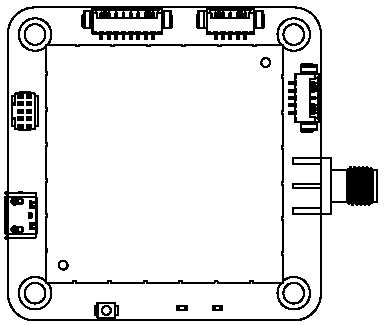
\includegraphics[]{swiftnav_v2_2_bottom.pdf}};
    % show origin
    %\fill (0,0) circle (2pt);
    
    % define destination coordinates
    \path (-0.1,1.875) coordinate (usb)
          (-0.1,3.625) coordinate (jtag)
          (2.16,5.55) coordinate (debug)
          (3.905,5.55) coordinate (uart1)
          (5.625,3.86) coordinate (uart2)
          (6.5,2.375) coordinate (sma);
          
    \node [below left of=usb, node distance=2.5cm] (usb_label) {Micro-USB};
    \draw[->] (usb_label) -| (usb);
    
    \matrix (jtag_pins) [pinoutmatrix, above of=usb_label, node distance=1.75cm] {
      |[pinnum]| 1 & |[fill=red!70]| 3.3V          & |[fill=cyan!70]| TMS      & |[pinnum]| 2 \\
      |[pinnum]| 3 & |[fill=black,text=white]| GND & |[fill=green!70]| TCK     & |[pinnum]| 4 \\
      |[pinnum]| 5 & |[fill=black,text=white]| GND & |[fill=yellow!70]| TDO    & |[pinnum]| 6 \\
      |[pinnum]| 7 & |[fill=black,text=white]| GND & |[fill=orange!70]| TDI    & |[pinnum]| 8 \\
      |[pinnum]| 9 & |[fill=black,text=white]| GND & |[fill=lightgray!70]| RST & |[pinnum]| 10 \\
    };
    \node [above of=jtag_pins, node distance=1.15cm] (jtag_label) {JTAG};
    \draw[->] (jtag_label) -| (jtag);
    \node [pin1, above of=jtag, node distance=1.2cm] {1};
    
    \matrix (debug_pins) [pinoutmatrix, above of=jtag_label, node distance=2cm, nodes={minimum width=2cm}] {
      |[pinnum]| 1 & |[fill=black,text=white]| GND \\
      |[pinnum]| 2 &  DEBUGB1 \\
      |[pinnum]| 3 &  DEBUGB2 \\
      |[pinnum]| 4 &  DEBUGB3 \\
      |[pinnum]| 5 &  DEBUGB4 \\
      |[pinnum]| 6 &  DEBUGB5 \\
      |[pinnum]| 7 &  DEBUGB6 \\
      |[pinnum]| 8 &  DEBUGB7 \\
    };
    \node [above of=debug_pins, node distance=1.65cm] (debug_label) {Debug Header};
    \draw[->] (debug_label) -| (debug);
    \node [pin1, right of=debug, node distance=2cm] {1};
    
    \node [right of=sma, node distance=2cm] (sma_label) {External Antenna};
    \draw[->] (sma_label) -- (sma);

    \node [right of=uart2, node distance=2cm] (uart2_label) {UART2};
    \matrix (uart2_pins) [pinoutmatrix, above of=uart2_label, node distance=1.15cm] {
      |[pinnum]| 1 & |[fill=black,text=white]| GND \\
      |[pinnum]| 2 & |[fill=orange!70]| RX \\
      |[pinnum]| 3 & |[fill=yellow!70]| TX \\
      |[pinnum]| 4 & |[fill=red!70]| 3.3V \\
      |[pinnum]| 5 & |[fill=red!70]| V+ \\
    };
    \node [pin1, below of=uart2] {1};
    \draw[->] (uart2_label) -- (uart2);
    
    \node [above of=uart2_pins, node distance=1.15cm] (uart1_label) {UART1};
    \draw[->] (uart1_label) -| (uart1);
    \node [pin1, right of=uart1] {1};

  \end{tikzpicture}
\end{center}

\begin{multicols}{2}
\raggedcolumns

\subsection*{USB}

Micro-USB socket provides USB connectivity to the host. This can be configured
as a USB-Serial bridge to the microcontroller or as a high-speed FIFO
interface to the SwiftNAP for streaming full-rate IF data samples to the host.

\subsection*{Active Antenna}

In addition to the on-board patch antenna an external active antenna input is
provided on an SMA connector for higher performance and system integration
flexibility.

\subsection*{JTAG}

0.05in pitch JTAG header allows access to SwiftNAP FPGA and microcontroller
JTAG chains for debugging.

\subsection*{Debug Header}

Provides access to debugging signals from the SwiftNAP. Assignment of these
signals varies depending on the SwiftNAP firmware loaded.

\subsection*{UARTs 1 \& 2}

Provide high-speed 3.3V LVTTL level UART interfaces which can be configured to
transmit NMEA or binary navigation solution data, system status and debugging
information and receive commands or differential corrections from the host or another
SwiftGNSS board.

\end{multicols}

\pagebreak

\section*{Electrical Specifications}

\begin{mpar}
\begin{multicols}{2}
  \noindent
  Supply voltage \dotfill 3.5 -- 5.5 V \\
  Power consumption \dotfill 600 mW\footnote{Typical, dependant on firmware configuration.} \\
  Current draw from 3.3V output \dotfill 500 mA max.\\
  Active antenna input impedance \dotfill 50 $\Omega$ \\
  Active antenna bias voltage \dotfill 3.3 V\footnote{Switchable in software}\\
  Active antenna current draw \dotfill 57 mA max.
\end{multicols}
\end{mpar}

\section*{Mechanical Drawing}
\begin{center}
  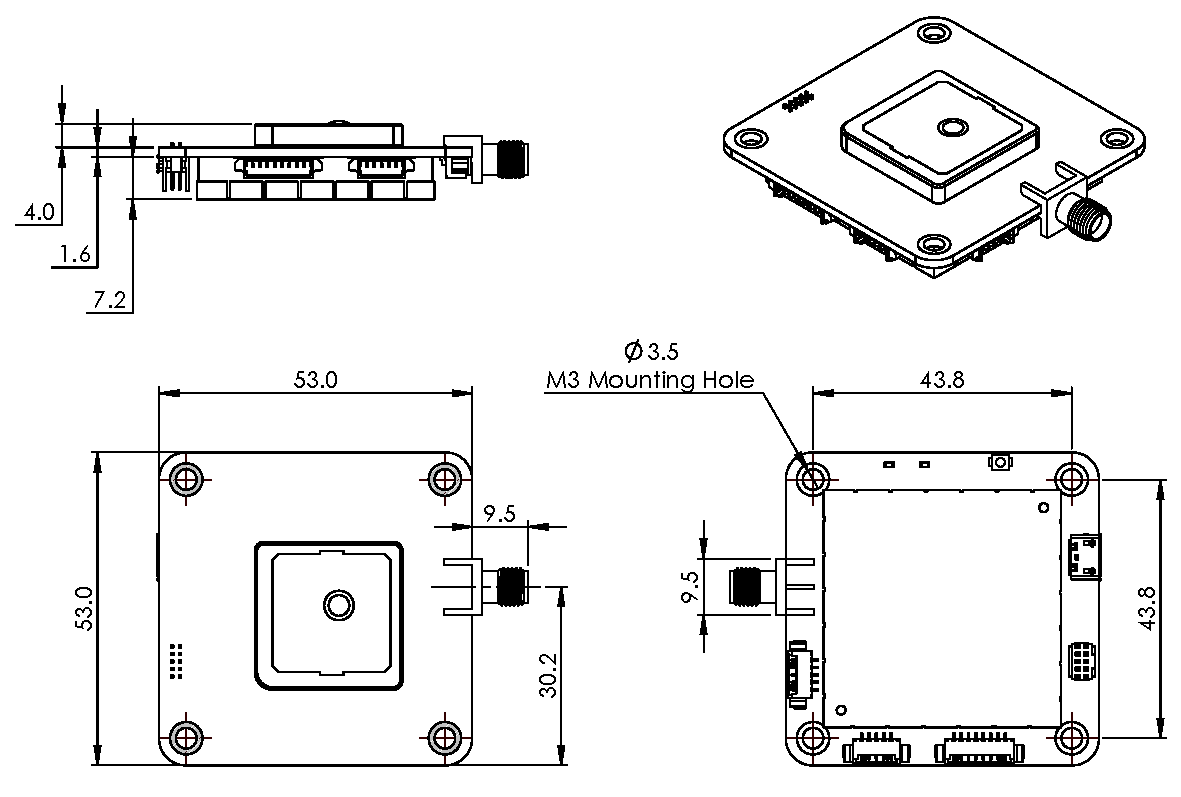
\includegraphics[scale=0.75]{swiftnav_v2_2_mechanical.pdf}
\end{center}

All dimensions are in millimeters. Drawing not to scale.

\subsection*{Notes}
\begin{enumerate}
  %\bulletnoindent
  \item Mass 25g.
  \item M3 mounting holes are plated through and connected internally to ground.
  \item 3D CAD models are available from our website, \url{http://www.swift-nav.com}.
\end{enumerate}




\end{document} 
